\section{Mělké neuronové sítě. Architektura, trénování a optimalizace}


\subsection*{Základní myšlenka neuronových sítí}

Neuronové sítě jsou modely inspirované propojením neuronů v mozku. V praxi jde o soustavu propojených
matematických funkcí, které transformují vstupní data na výstupní predikci.

V učení s učitelem se neuronová síť chápe jako parametrická funkce
\[
f_\theta:x\mapsto \hat{y},
\]
kde $\theta$ zahrnuje všechny váhy a biasy. Trénování znamená najít takové $\theta$, aby predikce $\hat{y}$
co nejlépe odpovídaly skutečným hodnotám $y$.

Zatímco lineární regrese používá jednu rovnici:
\[
\hat{y}=x^\top \beta,
\]
neuronová síť skládá více vrstev výpočtů:
\[
x \rightarrow \text{skrytá vrstva} \rightarrow \hat{y}.
\]

Neuronové sítě jsou použitelné pro:
\begin{itemize}
    \item regresi,
    \item binární klasifikaci,
    \item vícetřídní klasifikaci,
    \item rozpoznávání vzorů,
    \item obrazová, textová a časová data.
\end{itemize}

\subsection*{Mělká vs. hluboká neuronová síť}

\term{Mělká neuronová síť} má typicky:
\begin{itemize}
    \item vstupní vrstvu,
    \item jednu skrytou vrstvu,
    \item výstupní vrstvu.
\end{itemize}

\term{Hluboká neuronová síť} má více skrytých vrstev.

Mělké sítě mají menší výpočetní náročnost a jsou vhodné pro jednodušší úlohy. Hluboké sítě lépe zachycují
složité hierarchické vzory, například v obrazech nebo přirozeném jazyce.

\paragraph{Univerzální aproximační intuice.}
Jedna skrytá vrstva s dostatečným počtem nelineárních neuronů dokáže aproximovat velmi širokou třídu
spojitých funkcí. To neznamená, že je taková síť vždy prakticky nejlepší: může potřebovat mnoho neuronů,
hodně dat a opatrné ladění. Hluboké sítě často stejnou strukturu popíšou úsporněji, protože skládají jednodušší
reprezentace po vrstvách.

\subsection*{Perceptron}

Perceptron je základní stavební jednotka neuronové sítě.

Vstup:
\[
x=(x_1,\ldots,x_p).
\]

Váhy:
\[
w=(w_1,\ldots,w_p).
\]

Lineární kombinace vstupů:
\[
z
=
w^\top x + b
=
\sum_{j=1}^p w_jx_j+b.
\]

Výstup neuronu:
\[
a
=
\phi(z),
\]
kde $\phi$ je aktivační funkce.

\paragraph{Intuice.}
Váha $w_j$ říká, jak silně daný vstup ovlivňuje neuron. Bias $b$ posouvá rozhodovací hranici. Aktivační
funkce rozhoduje, jaký signál neuron pošle dál.

\begin{figure}[htbp]
  \centering
  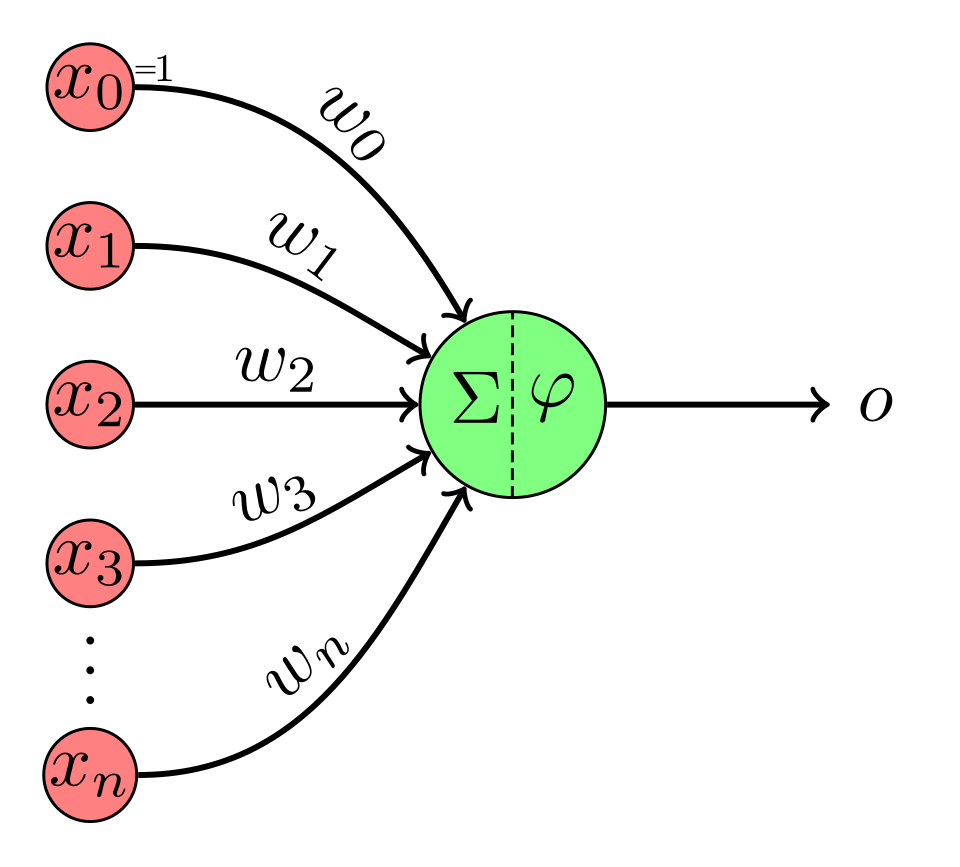
\includegraphics[width=0.68\linewidth]{assets/images/melke-neuronove-site/perceptron-unit.png}
  \caption[Perceptron jako umělý neuron]{Perceptron jako umělý neuron. Popis obrázku: vstupy se násobí
  vahami, sečtou se a výsledná hodnota projde aktivační funkcí. Bias lze chápat jako vstup s konstantní
  hodnotou $1$, který posouvá rozhodovací hranici. Zdroj obrázku: MartinThoma,
  \href{https://commons.wikimedia.org/wiki/File:Perceptron-unit.svg}{Wikimedia Commons}, licence CC0 1.0.}
  \label{fig:perceptron-unit}
\end{figure}

\subsection*{Perceptron pro binární klasifikaci}

U jednoduchého perceptronu se často používá skoková aktivační funkce:
\[
\phi(z)
=
\begin{cases}
1, & z\geq 0,\\
0, & z<0.
\end{cases}
\]

Predikce:
\[
\hat{y}
=
\phi(w^\top x+b).
\]

Perceptron vytváří lineární rozhodovací hranici:
\[
w^\top x+b=0.
\]

To znamená, že jednoduchý perceptron řeší pouze lineárně separovatelné úlohy.

\subsection*{Architektura mělké neuronové sítě}

Mělká dopředná síť s jednou skrytou vrstvou:

\[
x
\rightarrow
h
\rightarrow
\hat{y}.
\]

Pro $H$ neuronů ve skryté vrstvě:

\[
z_j^{(1)}
=
\sum_{\ell=1}^p
w_{j\ell}^{(1)}x_\ell
+
b_j^{(1)},
\qquad
j=1,\ldots,H.
\]

Aktivace skrytých neuronů:
\[
h_j
=
\phi(z_j^{(1)}).
\]

Výstupní vrstva:
\[
z^{(2)}
=
\sum_{j=1}^H
w_j^{(2)}h_j
+
b^{(2)}.
\]

Výstup:
\[
\hat{y}
=
g(z^{(2)}),
\]
kde $g$ závisí na typu úlohy.

Pokud je každá jednotka jedné vrstvy propojena se všemi jednotkami další vrstvy, mluví se o plně propojené
vrstvě. U tabulkových dat je to běžný výchozí model: vstupní proměnné nejprve vytvoří skryté reprezentace a
výstupní vrstva je převede na číselnou predikci nebo pravděpodobnosti tříd.

\begin{figure}[htbp]
  \centering
  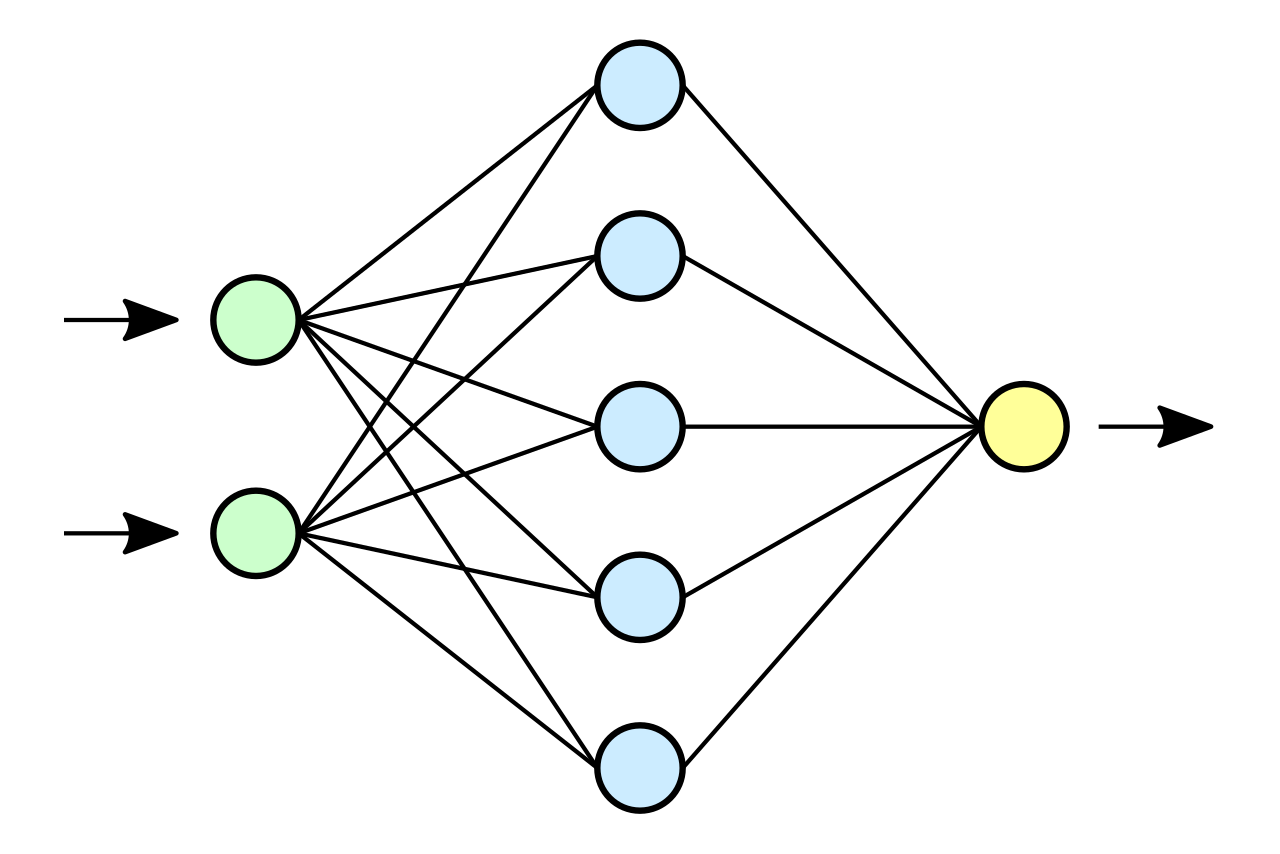
\includegraphics[width=0.74\linewidth]{assets/images/melke-neuronove-site/shallow-neural-network.png}
  \caption[Mělká dopředná neuronová síť]{Zjednodušené schéma dopředné neuronové sítě. Popis obrázku:
  signál teče zleva doprava ze vstupních proměnných přes skrytou vrstvu do výstupu. U mělké sítě je klíčová
  právě jedna skrytá vrstva; přidáním dalších skrytých vrstev vzniká hlubší architektura. Zdroj obrázku:
  Dake a Mysid, \href{https://commons.wikimedia.org/wiki/File:Neural\_network.svg}{Wikimedia Commons},
  licence CC BY 1.0.}
  \label{fig:shallow-neural-network}
\end{figure}

\subsection*{Maticový zápis}

Pro jednu skrytou vrstvu:

\[
h
=
\phi(W^{(1)}x+b^{(1)}),
\]

\[
\hat{y}
=
g(W^{(2)}h+b^{(2)}).
\]

Kde:
\begin{itemize}
    \item $W^{(1)}$ jsou váhy mezi vstupem a skrytou vrstvou,
    \item $b^{(1)}$ jsou biasy skryté vrstvy,
    \item $W^{(2)}$ jsou váhy mezi skrytou a výstupní vrstvou,
    \item $b^{(2)}$ je bias výstupní vrstvy.
\end{itemize}

\subsection*{Aktivační funkce}

Aktivační funkce zavádí nelinearitu. Bez nelineární aktivace by vícevrstvá neuronová síť byla jen lineární
model.

Dobrá aktivační funkce má být nelineární, numericky stabilní a ideálně má poskytovat použitelné gradienty
pro učení. V hidden vrstvách se dnes často používá ReLU nebo její varianty, zatímco sigmoid a softmax se
typicky objevují ve výstupní vrstvě klasifikačních modelů.

\begin{figure}[htbp]
  \centering
  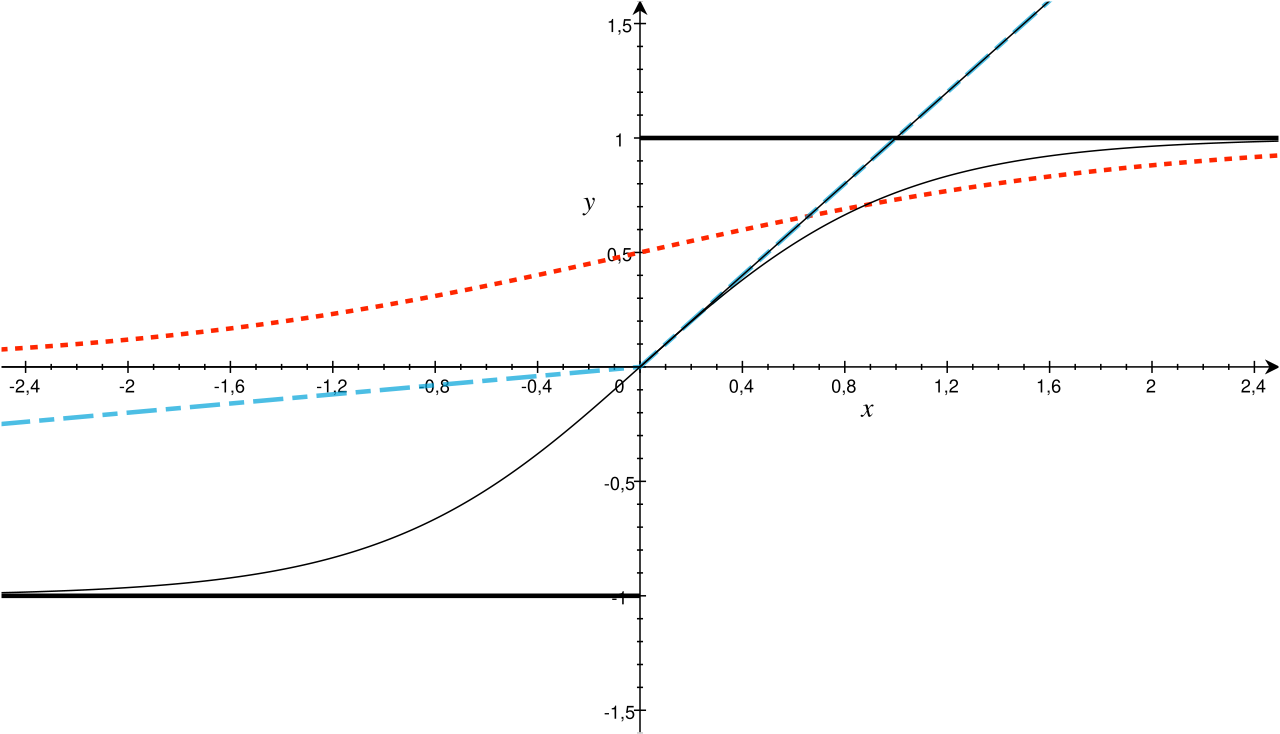
\includegraphics[width=0.86\linewidth]{assets/images/melke-neuronove-site/activation-functions.png}
  \caption[Aktivační funkce]{Příklady aktivačních funkcí. Popis obrázku: sigmoid převádí hodnoty do intervalu
  $(0,1)$, hyperbolický tangens do intervalu $(-1,1)$, ReLU propouští kladné hodnoty a záporné nastavuje na
  nulu. Volba aktivace ovlivňuje nelinearitu modelu i chování gradientů při trénování. Zdroj obrázku:
  Andreas Maier, Christopher Syben, Tobias Lasser a Christian Riess,
  \href{https://commons.wikimedia.org/wiki/File:ActivationFunctions.svg}{Wikimedia Commons}, licence CC BY 4.0.}
  \label{fig:activation-functions}
\end{figure}

\subsubsection*{Sigmoid}

\[
\sigma(z)=
\frac{1}{1+e^{-z}}.
\]

Vlastnosti:
\begin{itemize}
    \item výstup je v intervalu $(0,1)$,
    \item vhodná pro binární výstup,
    \item může trpět vanishing gradient problémem.
\end{itemize}

Derivace:
\[
\sigma'(z)
=
\sigma(z)(1-\sigma(z)).
\]

\subsubsection*{Tanh}

\[
\tanh(z)=
\frac{e^z-e^{-z}}{e^z+e^{-z}}.
\]

Výstup je v intervalu:
\[
(-1,1).
\]

\subsubsection*{ReLU}

\[
ReLU(z)=
\max(0,z).
\]

Výhody:
\begin{itemize}
    \item jednoduchá,
    \item rychlá,
    \item často dobře funguje,
    \item omezuje problém mizejících gradientů oproti sigmoidu.
\end{itemize}

Nevýhoda:
\begin{itemize}
    \item pro záporné hodnoty má nulový gradient, neuron může přestat učit.
\end{itemize}

\subsubsection*{Softmax}

Softmax se používá pro vícetřídní klasifikaci:
\[
\hat{p}_k
=
\frac{e^{z_k}}
{\sum_{\ell=1}^K e^{z_\ell}}.
\]

Platí:
\[
0\leq \hat{p}_k\leq 1,
\qquad
\sum_{k=1}^K \hat{p}_k=1.
\]

\subsection*{Volba výstupní vrstvy podle typu úlohy}

\begin{itemize}
    \item \textbf{Regrese:}
    lineární výstup
    \[
    \hat{y}=z.
    \]
    
    \item \textbf{Binární klasifikace:}
    sigmoid
    \[
    \hat{p}=P(y=1|x)=\sigma(z).
    \]
    
    \item \textbf{Vícetřídní klasifikace:}
    softmax
    \[
    \hat{p}_k=P(y=k|x).
    \]
\end{itemize}

\subsection*{Ztrátové funkce}

Neuronová síť se trénuje minimalizací ztrátové funkce:
\[
L(y,\hat{y}).
\]

Celková empirická ztráta:
\[
J(\theta)
=
\frac{1}{n}
\sum_{i=1}^n
L(y_i,\hat{y}_i),
\]
kde $\theta$ označuje všechny váhy a biasy v síti.

\subsubsection*{MSE pro regresi}

\[
L(y,\hat{y})
=
(y-\hat{y})^2.
\]

Celkově:
\[
MSE
=
\frac{1}{n}
\sum_{i=1}^n
(y_i-\hat{y}_i)^2.
\]

\subsubsection*{Binární cross-entropy}

Pro binární klasifikaci:
\[
L(y,\hat{p})
=
-
\left[
y\log(\hat{p})
+
(1-y)\log(1-\hat{p})
\right].
\]

\subsubsection*{Categorical cross-entropy}

Pro vícetřídní klasifikaci:
\[
L(y,\hat{p})
=
-
\sum_{k=1}^K
y_k\log(\hat{p}_k).
\]

\subsection*{Forward propagation}

Forward propagation znamená výpočet predikce od vstupu k výstupu.

Pro jedno pozorování:
\[
z^{(1)}=W^{(1)}x+b^{(1)},
\]
\[
h=\phi(z^{(1)}),
\]
\[
z^{(2)}=W^{(2)}h+b^{(2)},
\]
\[
\hat{y}=g(z^{(2)}).
\]

Potom spočítáme ztrátu:
\[
L(y,\hat{y}).
\]

\subsection*{Backpropagation}

Backpropagation je algoritmus pro efektivní výpočet gradientů ztrátové funkce podle všech vah a biasů.

Cílem je získat:
\[
\frac{\partial J}{\partial w}
\]
pro každou váhu $w$ v síti.

Používá se řetězové pravidlo:
\[
\frac{\partial L}{\partial w}
=
\frac{\partial L}{\partial \hat{y}}
\cdot
\frac{\partial \hat{y}}{\partial z}
\cdot
\frac{\partial z}{\partial w}.
\]

\paragraph{Intuice.}
Nejprve síť udělá predikci. Spočítáme chybu. Potom chybu propagujeme zpět sítí a zjišťujeme, které váhy
k chybě přispěly a jak je upravit.

Pro síť s jednou skrytou vrstvou lze zpětný průchod zapsat kompaktně. Označme chybu ve výstupní vrstvě:
\[
\delta^{(2)}
=
\frac{\partial L}{\partial z^{(2)}}.
\]
Gradienty pro výstupní vrstvu jsou:
\[
\frac{\partial L}{\partial W^{(2)}}=\delta^{(2)}h^\top,
\qquad
\frac{\partial L}{\partial b^{(2)}}=\delta^{(2)}.
\]
Chyba se do skryté vrstvy přenese přes váhy výstupní vrstvy:
\[
\delta^{(1)}
=
\left(W^{(2)\top}\delta^{(2)}\right)
\odot
\phi'(z^{(1)}),
\]
kde $\odot$ značí násobení po složkách. Gradienty pro první vrstvu jsou:
\[
\frac{\partial L}{\partial W^{(1)}}=\delta^{(1)}x^\top,
\qquad
\frac{\partial L}{\partial b^{(1)}}=\delta^{(1)}.
\]

U kombinace softmaxu a cross-entropy se výstupní chyba zjednoduší na tvar
\[
\delta^{(2)}=\hat{p}-y,
\]
což je jeden z důvodů, proč se tato dvojice v klasifikaci používá tak často.

\subsection*{Gradient descent}

Trénování znamená hledání vah, které minimalizují ztrátovou funkci:
\[
\min_{\theta} J(\theta).
\]

Gradient descent aktualizuje parametry proti směru gradientu:
\[
\theta^{(t+1)}
=
\theta^{(t)}
-
\eta
\nabla J(\theta^{(t)}).
\]

Kde:
\begin{itemize}
    \item $\eta$ je learning rate,
    \item $\nabla J(\theta)$ je gradient ztrátové funkce.
\end{itemize}

Pro jednu váhu:
\[
w^{(t+1)}
=
w^{(t)}
-
\eta
\frac{\partial J}{\partial w}.
\]

\paragraph{Intuice.}
Gradient ukazuje směr nejrychlejšího růstu ztráty. Proto se při minimalizaci pohybujeme opačným směrem.

Optimalizace neuronové sítě je zpravidla nekonvexní. Algoritmus proto nemusí najít globální minimum; v praxi
se hledá dostatečně dobré řešení, které dobře generalizuje na nová data. Důležité je sledovat nejen trénovací
ztrátu, ale i validační ztrátu.

\begin{figure}[htbp]
  \centering
  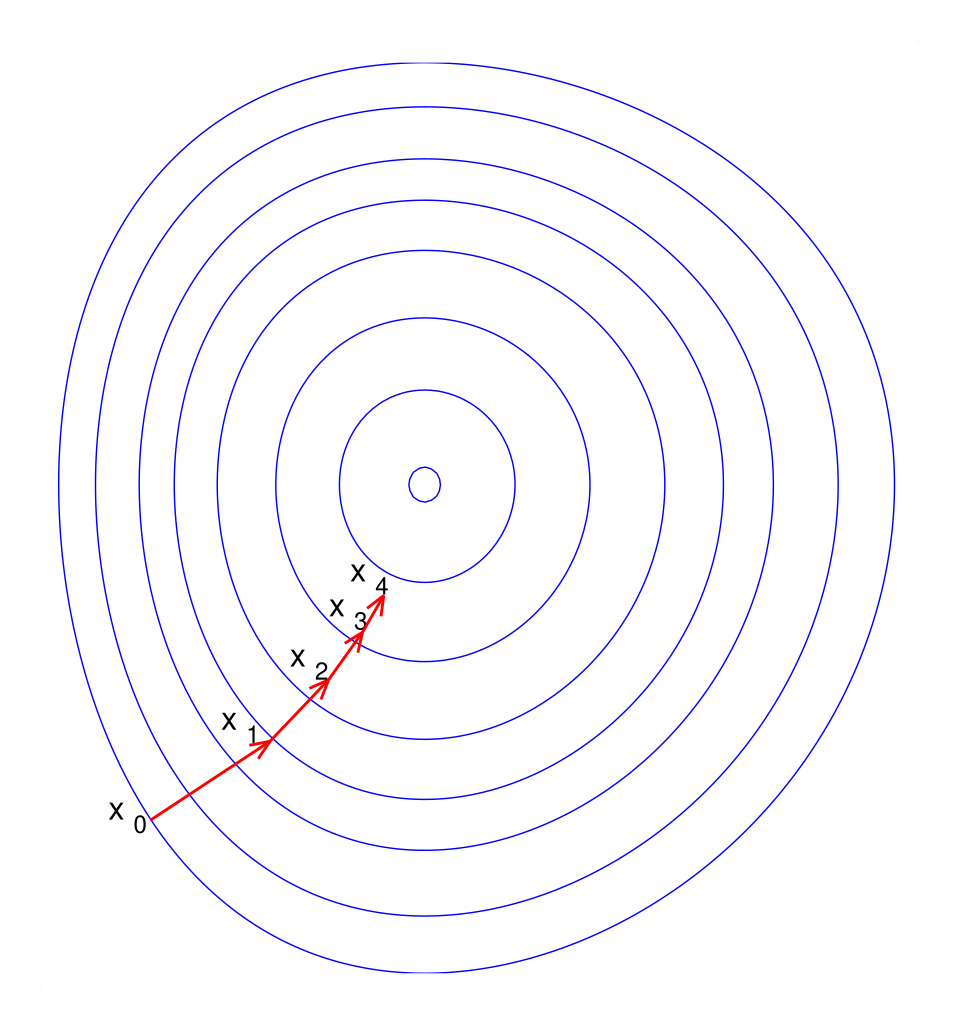
\includegraphics[width=0.58\linewidth]{assets/images/melke-neuronove-site/gradient-descent.png}
  \caption[Gradientní sestup]{Ilustrace gradientního sestupu. Popis obrázku: algoritmus postupně mění
  parametry ve směru, který snižuje hodnotu optimalizované funkce. U neuronových sítí se stejný princip
  používá pro aktualizaci vah podle gradientu ztrátové funkce. Zdroj obrázku: Zerodamage,
  \href{https://commons.wikimedia.org/wiki/File:Gradient\_descent.svg}{Wikimedia Commons}, public domain.}
  \label{fig:gradient-descent}
\end{figure}

\subsection*{Learning rate}

Learning rate $\eta$ určuje velikost kroku.

Pokud je $\eta$ příliš malé:
\begin{itemize}
    \item učení je velmi pomalé,
    \item model může potřebovat mnoho iterací.
\end{itemize}

Pokud je $\eta$ příliš velké:
\begin{itemize}
    \item optimalizace může oscilovat,
    \item ztráta nemusí klesat,
    \item algoritmus může divergovat.
\end{itemize}

\subsection*{Epochy, batch a mini-batch}

\begin{itemize}
    \item \textbf{Epoch:}
    jeden průchod celým trénovacím datasetem.
    
    \item \textbf{Batch:}
    část dat použitá pro jeden update vah.
    
    \item \textbf{Batch size:}
    počet pozorování v jedné dávce.
\end{itemize}

\subsection*{Varianty gradientního sestupu}

\subsubsection*{Batch gradient descent}

Používá celý dataset pro jeden update:
\[
\nabla J(\theta)
=
\frac{1}{n}
\sum_{i=1}^n
\nabla L_i(\theta).
\]

Výhody:
\begin{itemize}
    \item stabilní směr gradientu,
    \item hladší konvergence.
\end{itemize}

Nevýhody:
\begin{itemize}
    \item pomalé pro velká data,
    \item vysoká paměťová náročnost.
\end{itemize}

\subsubsection*{Stochastic gradient descent}

Používá jedno pozorování:
\[
\theta
\leftarrow
\theta
-
\eta
\nabla L_i(\theta).
\]

Výhody:
\begin{itemize}
    \item rychlé aktualizace,
    \item může pomoci uniknout z lokálních minim.
\end{itemize}

Nevýhody:
\begin{itemize}
    \item kolísavá konvergence,
    \item citlivost na learning rate.
\end{itemize}

\subsubsection*{Mini-batch gradient descent}

Používá malou dávku dat:
\[
B\subset \{1,\ldots,n\}.
\]

\[
\theta
\leftarrow
\theta
-
\eta
\frac{1}{|B|}
\sum_{i\in B}
\nabla L_i(\theta).
\]

Je to nejběžnější varianta v praxi.

\subsection*{Momentum}

Momentum vyhlazuje aktualizace a zrychluje pohyb ve stabilním směru.

\[
v_t
=
\gamma v_{t-1}
+
\eta \nabla J(\theta_t),
\]
\[
\theta_{t+1}
=
\theta_t-v_t.
\]

Momentum pomáhá omezit oscilace a zrychlit konvergenci.

\subsection*{Adaptivní optimalizátory}

\subsubsection*{AdaGrad}

AdaGrad upravuje learning rate pro každý parametr podle historie gradientů. Parametry s velkými gradienty
dostávají menší kroky.

\subsubsection*{RMSprop}

RMSprop používá exponenciálně vážený průměr čtverců gradientů, čímž řeší příliš rychlé snižování learning
rate u AdaGrad.

\subsubsection*{Adam}

Adam kombinuje momentum a adaptivní learning rate. Udržuje:
\begin{itemize}
    \item odhad prvního momentu gradientu,
    \item odhad druhého momentu gradientu.
\end{itemize}

Pro gradient $g_t=\nabla J(\theta_t)$ platí zjednodušeně:
\[
m_t=\beta_1m_{t-1}+(1-\beta_1)g_t,
\]
\[
v_t=\beta_2v_{t-1}+(1-\beta_2)g_t^2.
\]
Po korekci počátečního vychýlení se parametry aktualizují přibližně jako
\[
\theta_{t+1}
=
\theta_t
-
\eta
\frac{\hat{m}_t}{\sqrt{\hat{v}_t}+\varepsilon}.
\]

V praxi je Adam velmi často používaný optimalizátor.

\subsection*{Newtonova metoda a vztah k optimalizaci}

Newtonova metoda využívá nejen gradient, ale i druhou derivaci, tedy křivost funkce.

Pro jednu proměnnou:
\[
x_{t+1}
=
x_t
-
\frac{f'(x_t)}{f''(x_t)}.
\]

U více proměnných:
\[
\theta_{t+1}
=
\theta_t
-
H^{-1}
\nabla J(\theta_t),
\]
kde $H$ je Hessian.

Výhoda:
\begin{itemize}
    \item může konvergovat rychleji.
\end{itemize}

Nevýhody:
\begin{itemize}
    \item výpočet Hessianu je drahý,
    \item metoda je citlivá na počáteční hodnoty,
    \item u velkých neuronových sítí je často nepraktická.
\end{itemize}

Proto se v neuronových sítích používají hlavně gradientní metody, mini-batch trénování a optimalizátory jako
Adam.

\subsection*{Počet neuronů ve skryté vrstvě}

Počet neuronů je důležitý hyperparametr.

Příliš málo neuronů:
\[
\Rightarrow
\text{underfitting}.
\]

Příliš mnoho neuronů:
\[
\Rightarrow
\text{overfitting}.
\]

Praktický postup:
\begin{itemize}
    \item začít jednodušším modelem,
    \item postupně přidávat neurony,
    \item sledovat validační chybu,
    \item použít cross-validation nebo validační množinu.
\end{itemize}

\subsection*{Inicializace vah}

Váhy se typicky inicializují náhodně, ale ne příliš velké ani všechny stejné.

Pokud by všechny váhy byly stejné, neurony ve stejné vrstvě by se učily totéž. Náhodná inicializace rozbíjí
symetrii.

\subsection*{Regularizace a prevence přeučení}

Neuronové sítě se mohou snadno přeučit.

Možnosti prevence:
\begin{itemize}
    \item menší počet neuronů,
    \item regularizace vah,
    \item early stopping,
    \item dropout,
    \item více trénovacích dat,
    \item augmentace dat,
    \item validace na oddělených datech.
\end{itemize}

Dropout při trénování náhodně vypíná část neuronů, takže se síť nemůže příliš spoléhat na konkrétní jednotky.
Při predikci se používá celá síť se správným škálováním aktivací. U mělkých sítí se dropout používá méně
často než u hlubokých modelů, ale princip je důležitý: snižuje závislost modelu na jednotlivých vahách.

L2 regularizace:
\[
J_{\lambda}(\theta)
=
J(\theta)
+
\lambda
\sum_j w_j^2.
\]

L1 regularizace:
\[
J_{\lambda}(\theta)
=
J(\theta)
+
\lambda
\sum_j |w_j|.
\]

\subsection*{Early stopping}

Sledujeme chybu na validační množině:
\[
Err_{\text{val}}.
\]

Pokud trénovací chyba dál klesá, ale validační chyba začne růst, model se přeučuje.

\[
Err_{\text{train}}\downarrow
\quad
\text{a}
\quad
Err_{\text{val}}\uparrow
\quad
\Rightarrow
\quad
\text{zastavit trénování}.
\]

V praxi se nastavuje také \term{patience}, tedy kolik epoch bez zlepšení validační chyby ještě tolerujeme.
Early stopping je jednoduchá, ale silná regularizační technika, protože vybere model před začátkem výrazného
přeučení.

\subsection*{Vanishing a exploding gradient}

Vanishing gradient znamená, že gradienty při zpětné propagaci postupně mizí:
\[
\left|
\frac{\partial L}{\partial w}
\right|
\approx 0.
\]

Potom se váhy v dřívějších vrstvách učí velmi pomalu nebo vůbec. Problém je častější u hlubokých sítí a
aktivačních funkcí jako sigmoid nebo tanh.

Řešení:
\begin{itemize}
    \item ReLU a její varianty,
    \item vhodná inicializace vah,
    \item normalizace,
    \item reziduální architektury u hlubokých sítí.
\end{itemize}

U mělkých sítí je problém menší, ale princip je důležitý pro pochopení trénování.

Opačným problémem je \term{exploding gradient}, kdy jsou gradienty příliš velké a aktualizace vah začnou
divergovat. Pomáhá menší learning rate, vhodná inicializace, normalizace a u některých modelů také
\term{gradient clipping}, tedy omezení maximální velikosti gradientu.

\subsection*{Praktický workflow trénování}

\begin{enumerate}
    \item připravit data a odstranit/řešit missing values,
    \item zakódovat kategoriální proměnné,
    \item standardizovat numerické proměnné,
    \item rozdělit data na train/validation/test,
    \item zvolit architekturu sítě,
    \item zvolit aktivační funkce,
    \item zvolit loss function,
    \item zvolit optimalizátor a learning rate,
    \item trénovat model,
    \item sledovat train a validation chybu,
    \item ladit hyperparametry,
    \item finálně vyhodnotit na testovacích datech.
\end{enumerate}

U neuronových sítí je zvlášť důležité škálování vstupů. Standardizaci nebo normalizaci je potřeba naučit jen
na trénovacích datech a stejnou transformaci použít na validační a testovací data. Pokud by se scaler fitoval
i na testovací množině, šlo by o únik informace z testu do trénování.

\paragraph{Typické hyperparametry.}
\begin{itemize}
    \item počet neuronů ve skryté vrstvě,
    \item aktivační funkce,
    \item learning rate,
    \item batch size,
    \item počet epoch nebo early stopping,
    \item regularizační parametr,
    \item volba optimalizátoru.
\end{itemize}

\subsection*{Výhody a nevýhody mělkých neuronových sítí}

Výhody:
\begin{itemize}
    \item umí zachytit nelineární vztahy,
    \item použitelné pro regresi i klasifikaci,
    \item flexibilní architektura,
    \item základ pro pochopení hlubokého učení.
\end{itemize}

Nevýhody:
\begin{itemize}
    \item horší interpretovatelnost než regrese nebo stromy,
    \item nutnost ladit mnoho hyperparametrů,
    \item citlivost na škálování dat,
    \item riziko přeučení,
    \item optimalizace může skončit v horším lokálním řešení.
\end{itemize}

\subsection*{Co si pamatovat u zkoušky}

\begin{itemize}
    \item Perceptron je lineární kombinace vstupů, bias a aktivační funkce.
    \item Bez nelineární aktivace by síť byla jen lineární model.
    \item Mělká síť má jednu skrytou vrstvu; hluboká síť má více skrytých vrstev.
    \item Forward propagation počítá predikci, backpropagation počítá gradienty.
    \item Gradient descent a jeho varianty upravují váhy proti směru gradientu.
    \item Klasifikace obvykle používá cross-entropy, regrese MSE.
    \item Model je citlivý na škálování vstupů, learning rate a regularizaci.
\end{itemize}

\subsection*{Shrnutí ke zkoušce}

Mělká neuronová síť má vstupní vrstvu, jednu skrytou vrstvu a výstupní vrstvu. Každý neuron počítá lineární
kombinaci vstupů a aplikuje aktivační funkci:
\[
a=\phi(w^\top x+b).
\]

Díky aktivačním funkcím je síť schopna modelovat nelineární vztahy. Predikce se počítá dopředným průchodem
a chyba se minimalizuje pomocí ztrátové funkce. Backpropagation efektivně vypočítá gradienty a optimalizátor
upravuje váhy:
\[
w^{(t+1)}
=
w^{(t)}
-
\eta
\frac{\partial J}{\partial w}.
\]

Důležité jsou volba architektury, aktivačních funkcí, loss function, learning rate, optimalizátoru a prevence
přeučení. Mělké sítě jsou flexibilní, ale méně interpretovatelné a citlivé na správné nastavení.

\subsection*{Zdroje}

\begin{itemize}
    \item scikit-learn User Guide:
    \href{https://scikit-learn.org/stable/modules/neural\_networks\_supervised.html}{Neural network models
    (supervised)}.
    \item scikit-learn API Reference:
    \href{https://scikit-learn.org/stable/modules/generated/sklearn.neural\_network.MLPClassifier.html}{MLPClassifier}.
    \item Goodfellow, Bengio, Courville:
    \href{https://www.deeplearningbook.org/}{Deep Learning}.
    \item Wikimedia Commons:
    \href{https://commons.wikimedia.org/wiki/File:Perceptron-unit.svg}{Perceptron-unit}.
    \item Wikimedia Commons:
    \href{https://commons.wikimedia.org/wiki/File:Neural\_network.svg}{Neural network}.
    \item Wikimedia Commons:
    \href{https://commons.wikimedia.org/wiki/File:ActivationFunctions.svg}{ActivationFunctions}.
    \item Wikimedia Commons:
    \href{https://commons.wikimedia.org/wiki/File:Gradient\_descent.svg}{Gradient descent}.
\end{itemize}

\newpage
